\section{Deriving optima}
\newcommand{\gapShare}{15\xspace}
\newcommand{\gapShareMin}{9\xspace}
\newcommand{\gapShareMax}{21\xspace}
\newcommand{\gapOneShare}{9\xspace}
\newcommand{\topOneShare}{2.3\xspace}
\newcommand{\topTwelveShare}{15\xspace}
\newcommand{\topTwentyFourShare}{25\xspace}
\newcommand{\topSixtyFourShare}{52\xspace}
\newcommand{\splitsBeforePruning}{13\xspace}
\newcommand{\agreeRankOne}{99.9\xspace}
\newcommand{\agreeRankTwo}{86\xspace}
\newcommand{\agreeRankTwelve}{78\xspace}
\newcommand{\removedTwelve}{22\xspace}
\newcommand{\neighbourAgreeTwelve}{97\xspace}
\newcommand{\groupTwelveDocs}{124,689\xspace}
\newcommand{\groupTwelveShare}{12.5\xspace}
\newcommand{\groupTwelveNeighbours}{85\xspace}
\newcommand{\groupTwentyFourDocs}{9,305\xspace}
\newcommand{\groupTwentyFourNeighbours}{54\xspace}
\newcommand{\insideDocs}{325,353\xspace}
\newcommand{\insideAfterTwelve}{62,060\xspace}
\newcommand{\insideShareAfterTwelve}{19\xspace}
\newcommand{\insideNeighboursAfterTwelve}{84\xspace}
\newcommand{\keyFirstTwelveShare}{6.8\xspace}
\newcommand{\keyFirstTwelveDocs}{3,217\xspace}
\newcommand{\keyFirstTwelveNeighbours}{5\xspace}
\newcommand{\keyHeavyTwelveShare}{9.5\xspace}
\newcommand{\keyHeavyTwelveDocs}{302,372\xspace}
\newcommand{\keyHeavyTwelveNeighbours}{40\xspace}
\newcommand{\keyFirstEightShare}{5.2\xspace}
\newcommand{\probesEightyCfour}{72\xspace}
\newcommand{\docsEightyCfour}{18,107\xspace}
\newcommand{\docsShareEightyCfour}{1.8\xspace}
\newcommand{\probesNinetyCfour}{211\xspace}
\newcommand{\docsNinetyCfour}{52,164\xspace}
\newcommand{\docsShareNinetyCfour}{5.2\xspace}
\newcommand{\probesNinetyFiveCfour}{467\xspace}
\newcommand{\docsNinetyFiveCfour}{114,477\xspace}
\newcommand{\docsShareNinetyFiveCfour}{11.4\xspace}
\newcommand{\probesNinetyNineCfour}{1,330\xspace}
\newcommand{\docsNinetyNineCfour}{325,353\xspace}
\newcommand{\docsShareNinetyNineCfour}{32.5\xspace}
\newcommand{\probesEightyCeight}{127\xspace}
\newcommand{\docsEightyCeight}{15,615\xspace}
\newcommand{\docsShareEightyCeight}{1.6\xspace}
\newcommand{\probesNinetyCeight}{353\xspace}
\newcommand{\docsNinetyCeight}{42,847\xspace}
\newcommand{\docsShareNinetyCeight}{4.3\xspace}
\newcommand{\probesNinetyFiveCeight}{778\xspace}
\newcommand{\docsNinetyFiveCeight}{93,930\xspace}
\newcommand{\docsShareNinetyFiveCeight}{9.4\xspace}
\newcommand{\probesNinetyNineCeight}{2,440\xspace}
\newcommand{\docsNinetyNineCeight}{295,858\xspace}
\newcommand{\docsShareNinetyNineCeight}{29.6\xspace}

We now choose each method's settings for the dataset of Section~4: one million MS~MARCO
passages embedded with Nomic~v1.5, cut to 256 values and stored as 256 bits, with 200
queries and $K=100$. The requirement is the same for all three methods: return at least a
target share of the true top 100 (we use 80\%, 90\%, 95\% and 99\%), keep the index within
32~GB of RAM, and be as fast as possible. Memory turns out not to constrain anything here:
the largest index in Section~2 is under 100~MB. The choice is therefore made on time, and
each method may pick its own cluster count $C$, opened clusters $P$ and local settings. We
treat the methods one at a time and combine the results in Section~3.4.

\subsection{Original method}
Method A has two settings, $C$ and $P$, and one formula,
$T_A=T_{\rm route}(C,P)+c_{\rm call}+c_{\rm score}F_A(C,P)$. The recall requirement
removes one degree of freedom: for each $C$, $P$ must be the smallest number of clusters
that contains the target share of the reference documents. That number comes from the data.
We rank every cluster by its distance to each query, note the rank of the cluster that holds
each reference document, and read off how many clusters must be opened to reach each
target. Figure~\ref{fig:routing} shows the result as recall against documents opened, and
Table~\ref{tab:routing} lists the values at the four targets.

\begin{figure}[htb]\centering
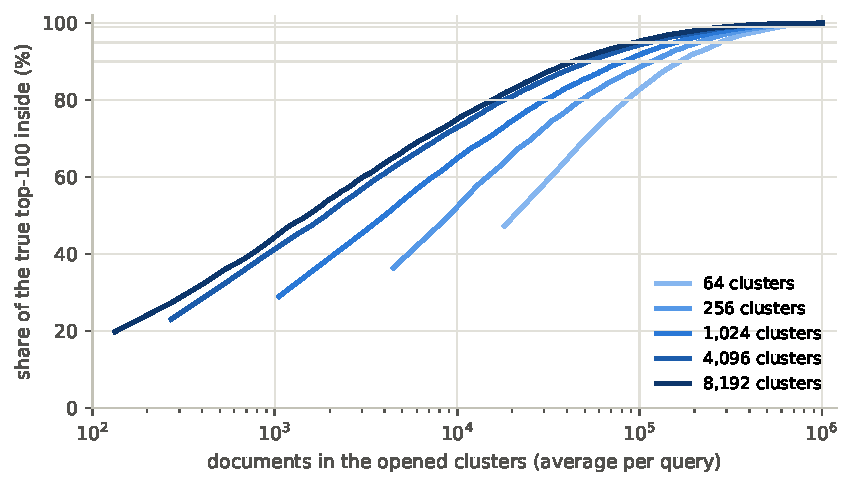
\includegraphics[width=.74\linewidth]{figures/routing.pdf}
\caption{Share of the true top-100 that lies in the opened clusters, against the number of
documents those clusters contain, for five cluster counts on the dataset. Horizontal lines
mark the four recall targets. More clusters reach a target with fewer documents, because the
opened region fits the query more tightly.}
\label{fig:routing}
\end{figure}

\begin{table}[htb]\centering\small
\caption{Clusters $P$ that must be opened, and documents those clusters hold on average,
for each recall target and cluster count. These are the $F_A$ values of the time formula.}
\label{tab:routing}
\begin{tabular}{@{}rrrrrrrrr@{}}\toprule
Clusters $C$ & \multicolumn{2}{c}{80\%} & \multicolumn{2}{c}{90\%} & \multicolumn{2}{c}{95\%} & \multicolumn{2}{c}{99\%}\\
 & $P$ & docs & $P$ & docs & $P$ & docs & $P$ & docs\\\midrule
64 & 6 & 98,610 & 11 & 178,239 & 18 & 286,892 & 37 & 580,487\\
256 & 12 & 50,005 & 29 & 118,453 & 52 & 211,419 & 119 & 480,127\\
1,024 & 31 & 30,626 & 84 & 82,157 & 164 & 160,584 & 420 & 412,040\\
4,096 & 72 & 18,107 & 211 & 52,164 & 467 & 114,477 & 1,330 & 325,353\\
8,192 & 127 & 15,615 & 353 & 42,847 & 778 & 93,930 & 2,440 & 295,858\\
\bottomrule\end{tabular}

\end{table}

Two effects pull in opposite directions as $C$ grows. The scoring term
$c_{\rm score}F_A$ falls, because Table~\ref{tab:routing} shows fewer documents for the
same recall: at 99\%, 574,000 documents with 64 clusters against 296,000 with 8,192.
The routing term rises, because selecting clusters compares the query with all $C$ centres,
$256C$ multiplications, and then sorts out the best $P$. Writing $T_{\rm route}\approx
c_{\rm centre}C+c_{\rm sort}P\log P$, the time is smallest where
\[
 \frac{dT_A}{dC}=c_{\rm centre}+c_{\rm score}\frac{dF_A}{dC}=0,
\]
that is, where opening one more cluster's worth of routing costs as much as the scoring it
saves. The recall curve flattens at high targets (the last few reference documents are
spread over many clusters), so $F_A$ stops falling quickly beyond a few thousand clusters,
while $c_{\rm centre}C$ keeps growing. With $c_{\rm score}\approx27$~ns per document
(Section~4) and a centre comparison of the same order, the formula puts the optimum at
$C=4{,}096$ or $8{,}192$ for every target: the difference in $F_A$ between them is worth
about 0.7~ms at 99\% and only 0.07~ms at 80\%, against roughly 0.1~ms of extra routing.
Section~4 measures both.

\subsection{Bitplanes}
Method B starts from the same clusters and adds two settings, the leaf size $L$ and the
node budget. At the same $C$ and $P$ the two time formulas differ by
\begin{equation}
 T_B-T_A=c_{\rm split}V_s+c_{\rm leaf}V_l+c_{\rm group}G-c_{\rm score}(F_A-F_B).
 \label{eq:bdiff}
\end{equation}
Method B wins only if the last term, the scoring it avoids, is larger than the three mask
terms. Two questions decide the size of $F_A-F_B$: how many documents does one split remove,
and may the removed group be skipped at all?

\textbf{How much a split removes.} A split keeps the documents whose bit agrees with the
query sign at one position. If document signs were balanced, half of a group would go each
way and twelve splits would cut a million documents to about 244. On this dataset the signs
are not balanced. Figure~\ref{fig:split} shows the share of documents removed by keeping the
preferred sign at each position, ordered by the query's weight. At the position with the
largest weight only \agreeRankOne\% of documents agree with the query and \(0.1\%\) are
removed; this position carries the same sign in almost every document and query, so it says
nothing about which documents are close. At the next eleven positions a split removes
between 14\% and \removedTwelve\%. After the twelve largest weights, \groupTwelveShare\% of
the collection is still in the group, \groupTwelveDocs\ documents instead of 244. Inside
the clusters opened for 99\% recall the effect is weaker still: those documents already
resemble the query, and twelve splits keep \insideShareAfterTwelve\% of them.

\begin{figure}[htb]\centering
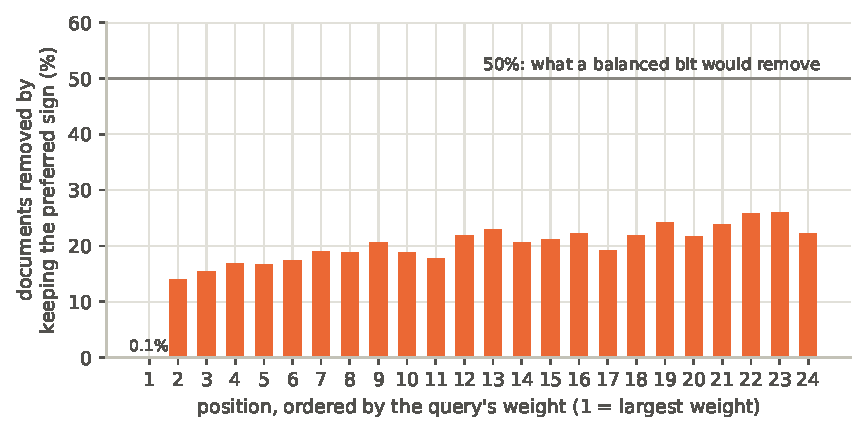
\includegraphics[width=.74\linewidth]{figures/split-removes.pdf}
\caption{What one split removes on this dataset, by the rank of the query weight at the
split position, averaged over the 200 queries. A balanced bit would remove 50\%. Real
embeddings agree with the query on its heavy positions far more often than not, so each
split removes a small minority.}
\label{fig:split}
\end{figure}

\textbf{Whether the removed group may be skipped.} Without a budget, method B drops a group
only when its penalty exceeds the gap $g$ (Section~2.3). On this dataset the gap averages
\gapShare\% of the total weight $Q$ (between \gapShareMin\% and \gapShareMax\% across
queries), while the largest single weight is only \topOneShare\% of $Q$ and the twelve
largest together are \topTwelveShare\%. A group that disagrees with the query at one heavy
position therefore has a penalty far below $g$, and the search must visit it. Adding up the
weights in order, a group would need to disagree at about \splitsBeforePruning\ of the
heaviest positions before the ceiling rule could drop it, and by then it holds almost
nothing. In the exact mode, then, $F_B=F_A$: every document that method A scores, method B
scores too, after paying for the masks. Equation~\ref{eq:bdiff} is minimised by making no
splits at all, $L\ge n_c$, which leaves
\[
 T_B-T_A=c_{\rm leaf}\sum_{c\ \text{opened}}W_c+c_{\rm group}P>0.
\]

\textbf{With a budget.} A node budget stops the search early and turns method B into an
approximate filter: it scores the groups that agree with the most heavy signs and drops the
rest, losing the reference documents in them. Whether that is a good trade depends on how
well ``agrees with the heavy signs'' predicts ``is a true neighbour'', compared with the
filter method A already has, ``is in a nearby cluster''. Figure~\ref{fig:filters} plots both
on the same axes: documents kept against true neighbours kept. Twelve splits keep
\groupTwelveShare\% of the documents and \groupTwelveNeighbours\ of the 100 neighbours;
opening the \probesEightyCfour closest of 4,096 clusters keeps \docsShareEightyCfour\%
of the documents and 80 neighbours. Clusters are the sharper filter at every point, so any
recall that a budget gives up is recovered more cheaply by opening fewer clusters. Method B
with a budget cannot beat method A here either.

\begin{figure}[htb]\centering
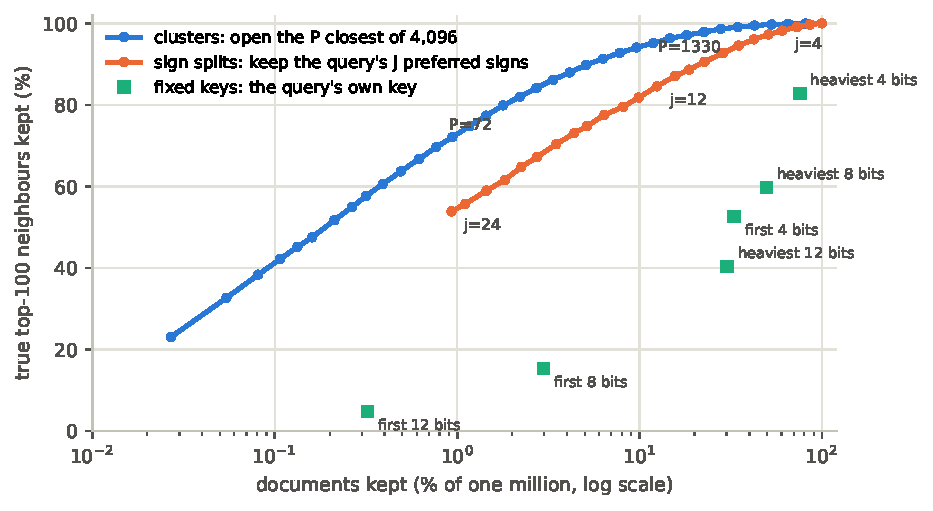
\includegraphics[width=.74\linewidth]{figures/filter-quality.pdf}
\caption{Three ways to keep only part of the collection, on the same dataset. A good filter
sits high and to the left: few documents kept, many true neighbours kept. Cluster selection
(blue) dominates sign splits (orange) and fixed keys (green) at every level.}
\label{fig:filters}
\end{figure}

\textbf{When Bitplanes would win.} The formula also says what a dataset must look like for
the mask work to pay. Two conditions are needed together: a split at a heavy position must
remove a large share of the group (balanced signs), and the heaviest few weights must
exceed the gap, $\sum_{i\le j}|q_{(i)}|>g$ for a small $j$, so that the ceiling drops the
other child. When both hold, one path of $j$ splits reads $jW$ words and scores about
$n2^{-j}$ documents; with $c_{\rm split}$ near half a nanosecond per word and
$c_{\rm score}$ near 27~ns per document, that path is cheaper than scoring the cluster as
soon as $j$ is a few units, by a factor that grows like $2^{j}$. Queries whose weight is
concentrated in a dozen positions that change from query to query are the case in which
method B is designed to shine. This dataset's queries spread their weight over hundreds of
positions.

\subsection{Backward Walk}
Method C adds the key width $h$. At the same clusters,
\begin{equation}
 T_C-T_A=c_{\rm lookup}H+c_{\rm key}E-c_{\rm score}(F_A-F_C),
\end{equation}
and the walk skips a key only when its penalty exceeds the gap $g$. The largest penalty a
key can have is the total weight of the $h$ key positions, so the question is whether those
fixed positions carry more than \gapShare\% of $Q$. They do not. The first eight positions
carry \keyFirstEightShare\% of the query weight on average and the first twelve
\keyFirstTwelveShare\%; even the twelve positions with the largest average weight across
all queries carry only \keyHeavyTwelveShare\%. No key is ever skipped, so the walk visits all
$2^h$ keys, $H=2^hP$, and $F_C=F_A$. The difference is minimised by the narrowest key:
$h=4$ costs $16P$ lookups on top of method A. Any wider key adds lookups without removing
scoring.

A limit on scored documents would make method C an approximate filter, like a budget for
method B. Figure~\ref{fig:filters} shows how the query's own key performs in that role.
With the first twelve positions as the key, the query's key holds \keyFirstTwelveDocs\
documents but only \keyFirstTwelveNeighbours\ of the 100 true neighbours: a key built from
light positions selects documents that agree where it hardly matters. With the twelve
heaviest positions, the key holds \keyHeavyTwelveDocs\ documents and
\keyHeavyTwelveNeighbours\ neighbours, because those positions are the ones almost every
document shares. Either way the key is a far worse filter than the clusters, so a candidate
limit cannot make method C competitive on this dataset.

\textbf{When Backward Walk would win.} Method C needs what method B needs, with one more
condition: the heavy positions must be the same for every query, because the key positions
are fixed when the index is built. Given that, a directory lookup is cheaper than a mask
split, and method C would reach the small group in one lookup where method B needs $h$
splits.

\subsection{Comparison}
Table~\ref{tab:conditions} collects the conditions and the dataset's values.
Both new methods can only remove scoring work when a small set of query positions is heavy
enough to exceed the gap and balanced enough to split the documents. On this dataset
neither condition holds, so the formulas predict, for every recall target, the order
\[
 T_A<T_B\ (\text{no splits})<T_C\ (h=4),
\]
with method B and C behind by their bookkeeping only: about $c_{\rm leaf}\sum W_c+
c_{\rm group}P$ for B and $16\,c_{\rm lookup}P$ for C. At the 99\% target with $C=4{,}096$
and $P=\probesNinetyNineCfour$, those are fractions of a millisecond on top of about
$c_{\rm score}\times\docsNinetyNineCfour\approx9$~ms of scoring. Table~\ref{tab:regions}
states where each method is expected to be fastest in general. Section~4 tests the
prediction for this dataset.

\begin{table}[htb]\centering\small
\caption{What each new method needs in order to skip scoring work, and what this dataset
provides. $g$ is the gap of Table~\ref{tab:symbols}, averaged over queries.}
\label{tab:conditions}
\begin{tabularx}{\linewidth}{@{}YlYc@{}}\toprule
Condition & Needed by & This dataset & Met\\\midrule
Heaviest few weights exceed the gap: $\sum_{i\le j}|q_{(i)}|>g$ for small $j$ & B and C & 12 heaviest weights: \topTwelveShare\% of $Q$; gap: \gapShare\% of $Q$; \splitsBeforePruning\ positions needed & no\\
A split on a heavy position removes about half the group & B and C & removes 0.1\% at the heaviest position, 14--\removedTwelve\% at the next eleven & no\\
The heavy positions are the same for every query & C only & first 12 positions: \keyFirstTwelveShare\% of $Q$; 12 heaviest on average: \keyHeavyTwelveShare\% & no\\
A cluster boundary is a weak filter, so local pruning has work left to save & B and C & \probesEightyCfour of 4,096 clusters hold 80 of 100 neighbours in \docsShareEightyCfour\% of the documents & no\\\bottomrule
\end{tabularx}
\end{table}

\begin{table}[htb]\centering\small
\caption{Where each method is expected to be fastest, from the formulas of Section~2.}
\label{tab:regions}
\begin{tabularx}{\linewidth}{@{}lY@{}}\toprule
Fastest & Situation\\\midrule
A: original & Query weight is spread over many positions, or documents mostly share the query's sign at its heavy positions. No group or key can be dropped, so extra structure only adds work. This dataset.\\
B: bitplanes & A few heavy positions carry more weight than the gap, their signs split the documents evenly, and which positions are heavy changes from query to query. Splits follow each query's own order.\\
C: backward walk & The same as B, but the heavy positions are the same for all queries, so a fixed key captures them and one lookup replaces several splits.\\\bottomrule
\end{tabularx}
\end{table}
